\begin{frame}{Agenda}
\begin{itemize}
    \item Introduction
    \item \textbf{Literature Review}
    \item Methodology
    \item Results
    \item Conclusion and Future Work
\end{itemize}
\end{frame}

%%

\begin{frame}{Literature Review} \pause
    Recommender Systems\\ \pause
    \vspace{0.5cm}
    Clustering\\ \pause
    \vspace{0.5cm}
    Principal Component Analysis (PCA)
\end{frame}

%%

\begin{frame}{Recommender Systems} \pause
    \begin{column}{.4\linewidth}
        Collaborative filtering \pause
        \begin{itemize}
            \item "people like you also like X"
            \item "if you like X  you may like Y"
        \end{itemize}
    \end{column} \pause
    \begin{column}{.6\linewidth}
        \begin{figure}
           \centering
           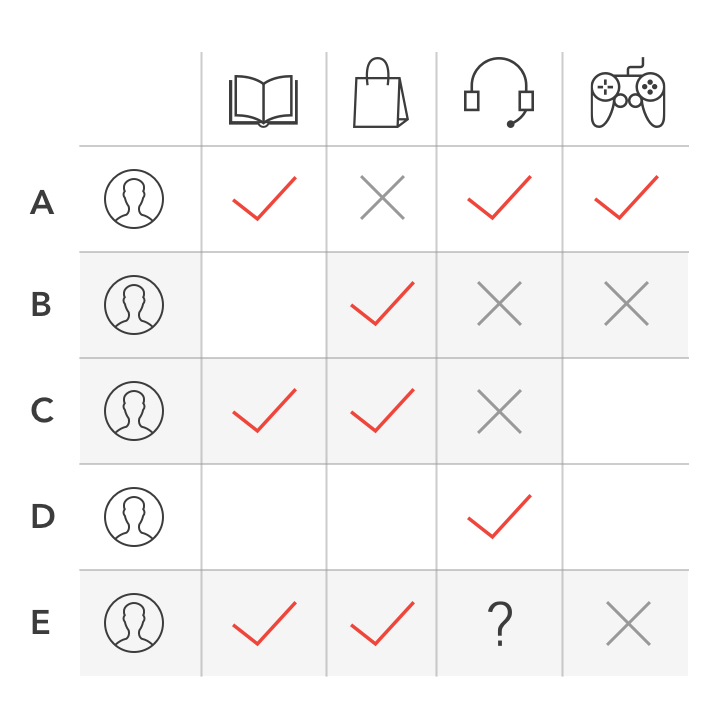
\includegraphics[width=6cm]{fig/ch2-colab-filt-user-user.jpg}
           \caption{User-based logic on collaborative filtering}
        \end{figure}
    \end{column}
\end{frame}

\begin{frame}{Recommender Systems}
    \begin{column}{.4\linewidth}
        Content-based filtering \pause
        \begin{itemize}
            \item user profile \pause
        \end{itemize}
    \end{column}
    \begin{column}{.6\linewidth}
        \begin{figure}
           \centering
           \caption{Content-based example}
           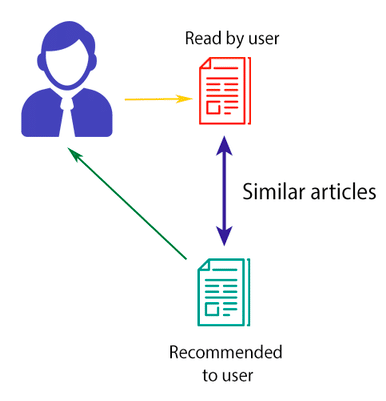
\includegraphics[width=.65\linewidth]{fig/content-based-example.png}
        \end{figure}
    \end{column}
\end{frame}

%%

\begin{frame}{Recommender Systems - Lift} \pause
    \begin{figure}
        \caption{Rectangular box with colored balls.} \pause
        \begin{subfigure}{\linewidth}
            \centering
            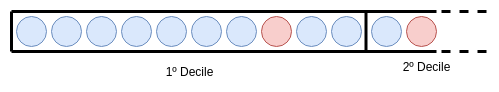
\includegraphics[width=\linewidth]{fig/ch2-rec-box-upper.png}
            \caption{Upper view.}
        \end{subfigure}
        \begin{subfigure}{\linewidth}
            \centering
            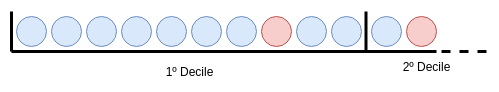
\includegraphics[width=\linewidth]{fig/ch2-rec-box-front.png}
            \caption{Front view.}
        \end{subfigure}
    \end{figure}
\end{frame}

%%

\begin{frame}{Recommender Systems - Lift}
    \begin{figure}
        \caption{Reordering of the balls.} \pause
        \begin{subfigure}{\linewidth}
            \centering
            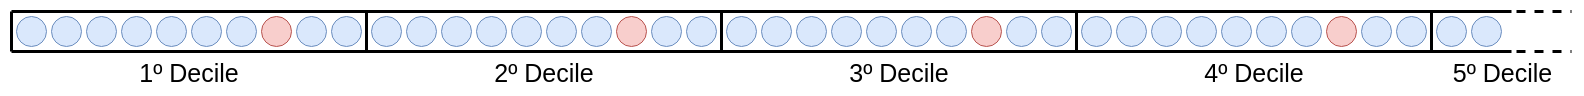
\includegraphics[width=\linewidth]{fig/ch2-rec-box-ordering-before.png}
            \caption{Before.} \pause
        \end{subfigure}
        \begin{subfigure}{\linewidth}
            \centering
            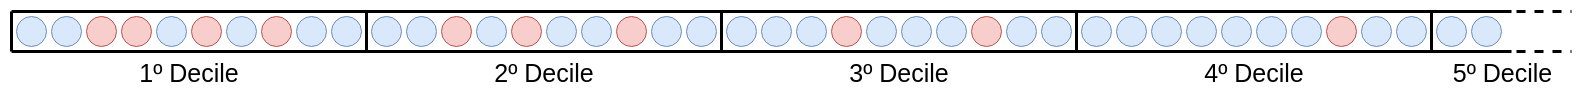
\includegraphics[width=\linewidth]{fig/ch2-rec-box-ordering-after.png}
            \caption{After.}
        \end{subfigure}
    \end{figure}
\end{frame}

%%

\begin{frame}{Recommender Systems - Lift}
    \begin{figure}
       \centering
       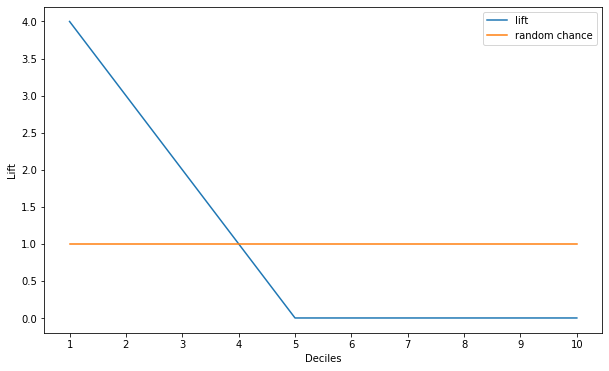
\includegraphics[width=\linewidth]{fig/ch2-lift-plot.png}
       \caption{Lift plot for the reordered box with the random chance.}
    \end{figure}
\end{frame}

%%

\begin{frame}{Recommender Systems - Lift} \pause
    \begin{column}{.5\textwidth}
        Market: $\mathcal M$ with size $|\mathcal M |\!=\!N$ \\ \pause
        \vspace{0.25cm}
        Leads: $\mathcal L \supset \mathcal M $, with $|\mathcal L|\!=\!n$ \\ \pause
        \vspace{0.25cm}
        $\mathcal L$ is unknown! \\ \pause
    \end{column}
    \begin{column}{.5\textwidth}
        Random chance: $n/N$ \\ \pause
        \vspace{0.25cm}
        Company $X_i$ -> score $S_i$ \\ \pause
        \vspace{0.25cm}
        Ordered: $S_i>S_{i-1}$ from $S_N$ to $S_1$ \\ \pause
    \end{column}
    \vfill
    \begin{column}{\textwidth}
        Given a $k$: \pause
        \vspace{0.25cm}
        \LARGE{
            \begin{equation*}
                \mathrm{lift}_k = \frac{P(X_{i:k\leq i\leq N}\in \mathcal L)}{n/N}
            \end{equation*}
        }
    \end{column}
\end{frame}

%%

\begin{frame}{Clustering} \pause
    \vspace{0.2cm}
    \begin{column}{\linewidth}
        Unsupervised learning technique \\ \pause
        \vspace{0.2cm}
        "Hidden" structures/patterns in a dataset \\ \pause
    \end{column}
    \begin{column}{\linewidth}
        \begin{figure}
            \centering
            \caption{Visualization of clusters}
            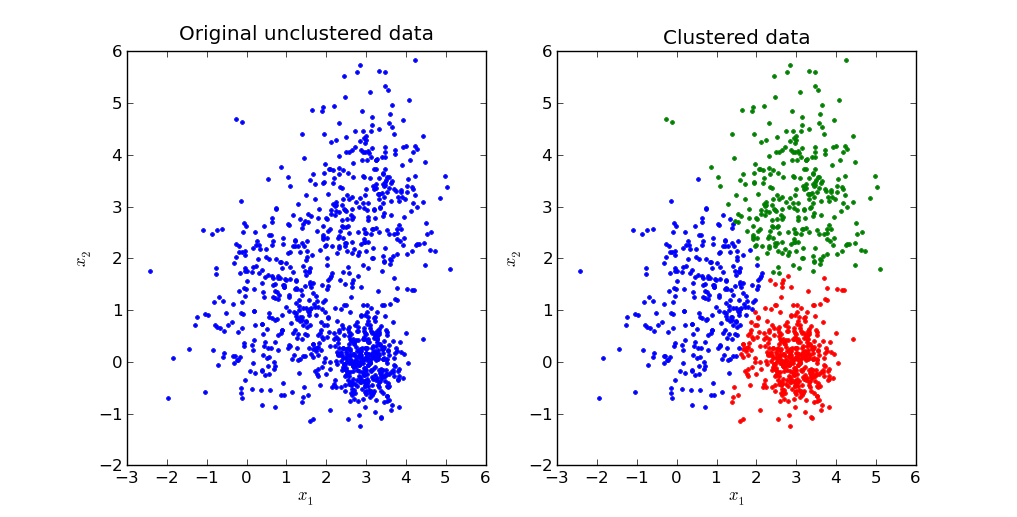
\includegraphics[width=.8\linewidth]{fig/clustering-example.png}
        \end{figure}
    \end{column}
\end{frame}

%%

\begin{frame}{PCA}
    \begin{column}{.5\linewidth}
        \onslide<2->{Orthogonal linear transformation \\}
        \vspace{0.5cm}
        \onslide<3->{Principal Components} \onslide<4->{ -> original data variance} \\
        \vspace{0.5cm}
        \onslide<6->{Dimensionality reduction \\}
        \vspace{0.5cm}
        \onslide<7->{PCA plot}
    \end{column} 
    \begin{column}{.5\linewidth}
    \onslide<5->{
        \begin{figure}
           \centering
           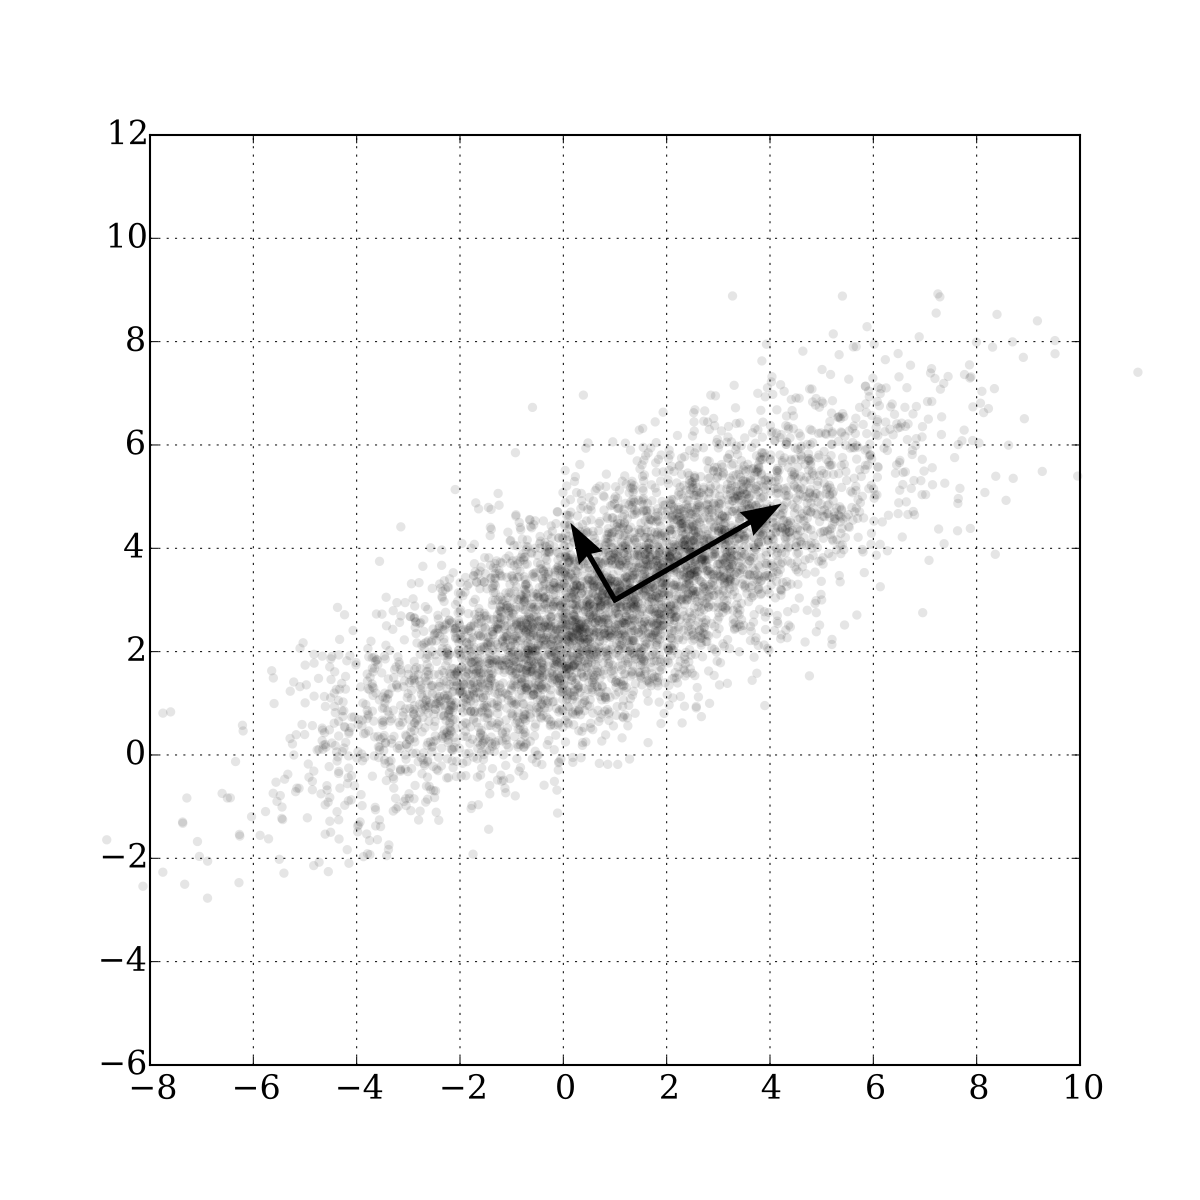
\includegraphics[width=6cm]{fig/pca-example.png}
           \caption{Principal components of a dataset}
        \end{figure}
    }
    \end{column}
\end{frame}
